\chapter{Marco Teórico y objetivos del trabajo}\label{capitulo_1}
\iffalse
\begin{chapquote}{Autor, \textit{tiempo}}
`` cita''
\end{chapquote}
\fi

En el presente capítulo se muestra en primer lugar el marco de desarrollo del Trabajo Fin de Máster. A continuación, se presenta un cuadro teórico que pretende exponer un conocimiento básico sobre el sistema nervioso central
en seres humanos relacionado con la médula espinal, así como las posibles lesiones que puede sufrir
y su clasificación. 
\\
\\
Una vez comprendido este marco teórico, se tratará el tema principal del presente trabajo: la neuro-rehabilitación
de la marcha patológica en el ser humano y las tecnologías disponibles para ello. 
\\
\\
Por último, se expondrá y explicará el conjunto de objetivos que se pretende alcanzar tras la finalización del trabajo.


\section{Marco de desarrollo}
El presente Trabajo Fin de Máster se ha realizado en un ambiente laboral: el autor lo ha desarrollado trabajando en el equipo de neuro-rehabilitación del Insituto Cajal\cite{equipo_cajal}, perteneciente al Consejo Superior de Investigaciones Científicas (CSIC). Esta oportunidad implica la aplicación de conocimientos adquiridos durante el Máster de Electrónica Industrial (MEI) y el Grado en Ingeniería en Tecnologías Industriales (GITI) de forma práctica. 
\\
\\
El ámbito de desarrollo del trabajo es por tanto la investigación científica en el campo de la salud. Éste se centra en el estudio del sistema nervioso central, los posibles daños que puede sufrir causados por lesiones medulares e ictus y su rehabilitación. En concreto, se trata la neuro-rehabilitación de la marcha patológica ya que, entre otras consecuencias, los daños en el sistema nervioso central implican pérdidas totales y/o parciales de habilidades motrices y sensoriales. Estas consecuencias dificultan o imposibilitan el ciclo de marcha en el ser humano impidiendo la realización de ejercicios como caminar, subir escaleras o sentarse y dando lugar, en efecto, a la marcha patológica.
\\
\\
Sin embargo, este tipo de neuro-rehabilitación presenta un conjunto de limitaciones inherentes a las diferentes técnicas de las que se sirve. Se parte de ejercicios elaborados y llevados a cabo por equipos multidisciplinares de profesionales en centros especializados. Aún así, el uso de terapeutas en neuro-rehabilitación tiene limitaciones como el cansancio y fuerza y repetibilidad insuficientes. Es por ello principalmente por lo que entran en juego tecnologías como el uso de exoesqueletos robóticos y la electroestimulación muscular. No obstante, estas tecnologías también presentan desventajas como por ejemplo el coste y la fatiga muscular, respectivamente.
\\
\\
De este modo, se tiene presente como única motivación la mejora de la calidad de vida de los pacientes que padecen de una marcha patológica debido a lesiones en el sistema nervioso central. Para ello sirve pues la neuro-rehabilitación, es decir, para mitigar las consecuencias que implican estas lesiones y potenciar el nivel de independencia de los pacientes en la realización de tareas diarias.
\\
\\
Por lo tanto, el objetivo principal del presente Trabajo Fin de Máster es el estudio, combinación y mejora de las diferentes tecnologías disponibles en la neuro-rehabilitación de marcha patológica. Esto se lleva a cabo en el proceso de construcción de una prótesis híbrida en el que el autor del presente trabajo participa. Este tipo de prótesis combina dichas tecnologías, reduce sus limitaciones y potencia sus ventajas.
\\
\\
Una vez visto el marco en el que se desarrolla el trabajo, antes de abordar con mayor claridad los objetivos que pretende alcanzar es necesario revisar una serie de conceptos sobre el sistema nervioso central en seres humanos, así como las tecnologías disponibles para la neuro-rehabilitación. En concreto, se tratarán las lesiones medulares y no el ictus para poder así profundizar en campo fisiológico de la médula espinal, los tipos de lesiones que puede sufrir y su neuro-rehabilitación. Además, la médula espinal es un elemento de vital importancia en el sistema nervioso central ya que otorga capacidades como el movimiento, la locomoción, sensibilidad, sensación de equilibrio y percepción de posición del cuerpo además del uso voluntario de otros órganos.

\section{La médula espinal}
La médula espinal es una estructura neurológica larga, fina y cilíndrica que se extiende desde la base del cráneo hasta el espacio entre la primera y segunda vértebra lumbar\cite{anatomia_medula_1}\cite{anatomia_medula_2}. Sus principales funciones implican la transmisión de información motora a los músculos, la recepción de información sensorial hacia el cerebro y la coordinación de reflejos. Está contenida en la columna vertebral aunque se extiende más allá de esta protección ósea. En seres humanos la columna vertebral tiene una longitud de entre 70 y 75 cm y se compone por 31 vértebras agrupadas en 5 secciones: 8 cervicales, 12 torácicas, 5 lumbares, 5 sacrales y el coxis tal y como se aprecia en la figura \ref{fig:columna_vertebral}\\

\begin{figure}[!htb]
\centering
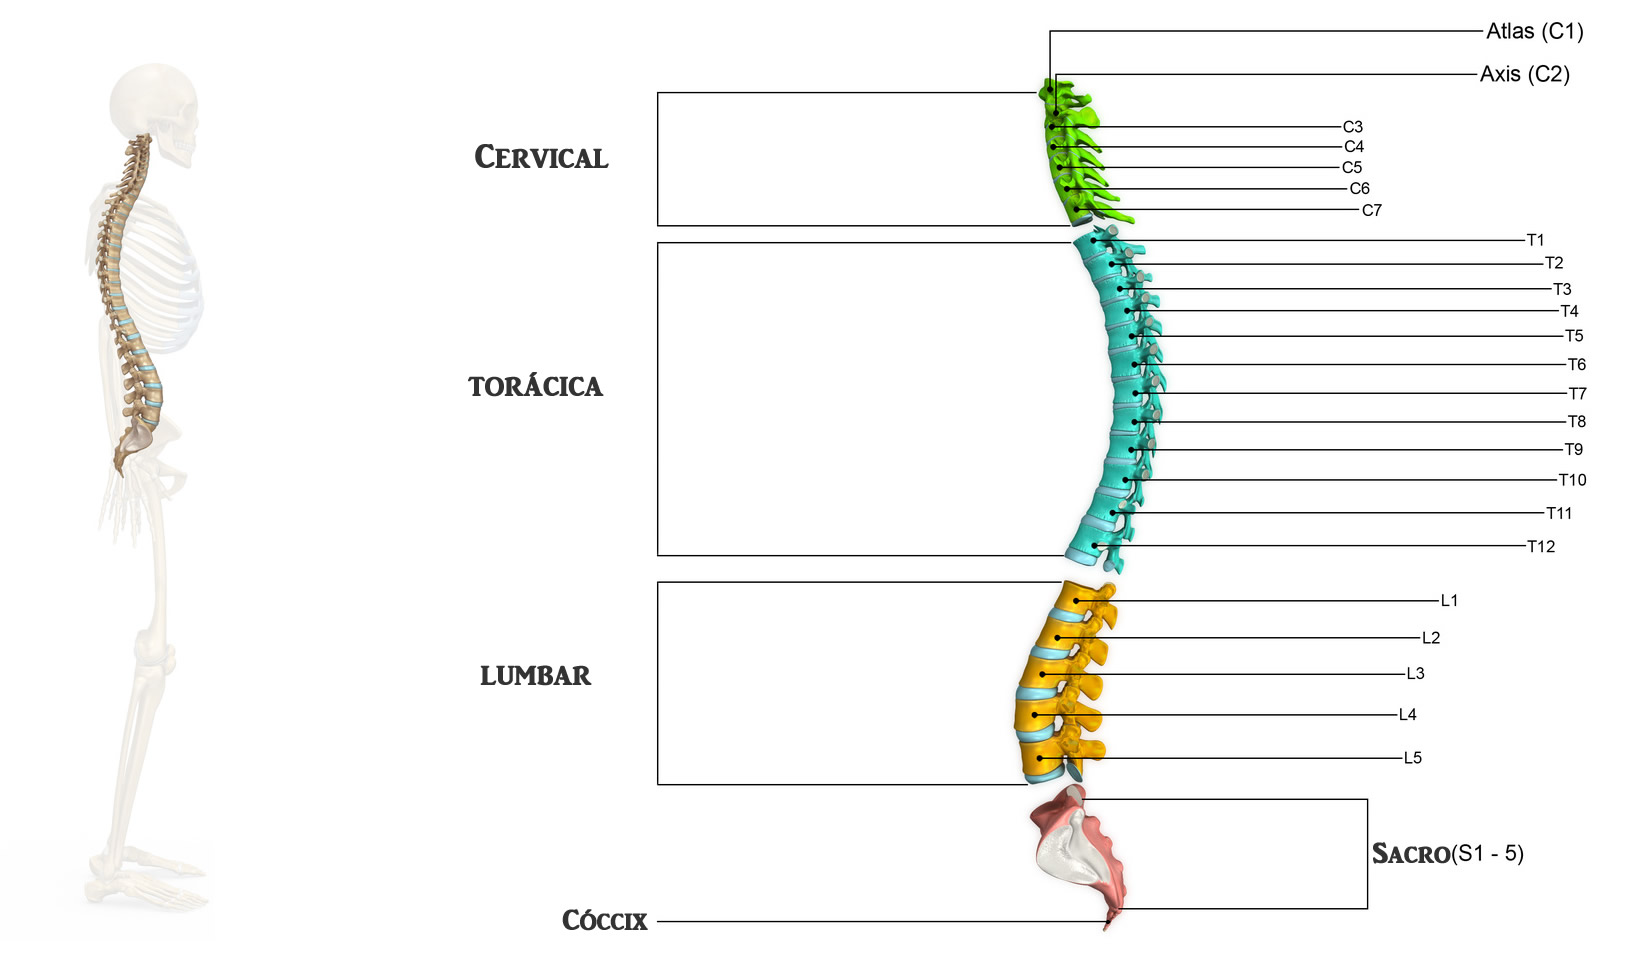
\includegraphics[scale=0.8]{columna_vertebral}
  \caption{Representación de la columna vertebral es sus 5 secciones\cite{columna_vertebral}.}\label{fig:columna_vertebral}
\end{figure}

Al igual que la columna vertebral, la médula espinal está organizada en 5 secciones de 31 segmentos en total: 8 cervicales, 12 torácicos, 5 lumbares, 5 sacrales y el nervio del coxis. Tiene una longitud total de entre 40 y 45 cm y cada segmento está asociado a dos nervios espinales, derecho e izquierdo. Este conjunto de nervios forman los nervios sensoriales, que entran en la médula espinal en cada segmento recibiendo información sensorial, y los nervios motores, que emergen de la misma y transmiten la información necesaria a los músculos para que éstos actúen en consecuencia.\cite{anatomia_medula_1}
\\
\\
Cada nervio espinal se compone de fibras nerviosas inervadas a miotomas (áreas musculares) y dermatomas (áreas de la piel)\cite{sci_clasificacion} siendo estos últimos fácilmente localizables en la superficie del cuerpo según se aprecia en la figura \ref{fig:dermatomas}\\

\begin{figure}[!htb]
\centering
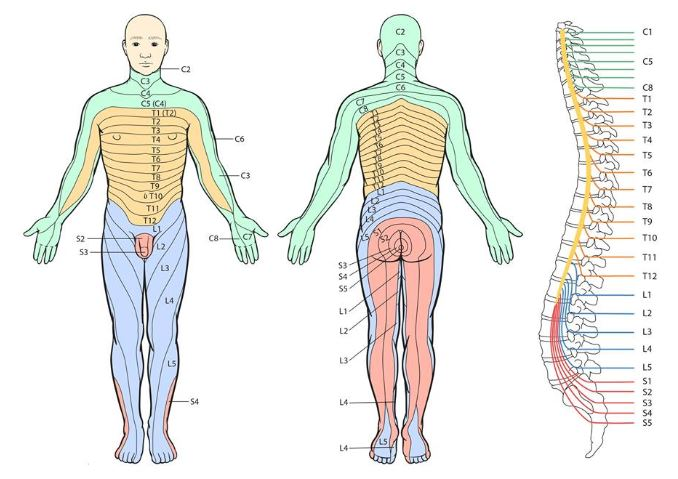
\includegraphics[scale=0.6]{dermatomas}
  \caption{Representación de dermatomas y su conexión con la médula espinal\cite{dermatomas}.}\label{fig:dermatomas}
\end{figure}


En lo que a miotomas o conjuntos de músculos se refiere, los segmentos cervicales están involucrados en la respiración y movimientos de cabeza, cuello y brazos. La sección torácica se encarga del control de dedos, pecho, espalda y abdomen. Por último, las secciones lumbar y sacral están asociadas con el control de músculos involucrados en la locomoción, micción, función intestinal y funciones reproductivas. 
\\
\\
Un análisis más profundo de la médula espinal conlleva estudiar su sección transversal. Esto revela un núcleo de materia gris en forma de mariposa o H rodeado de materia blanca. La materia gris está formada por neuronas motoras y sensoriales cada una con sus axones (prolongación de la neurona encargada de la transmisión de impulsos nerviosos) Por otra parte, la materia blanca está formada por fibras nerviosas que se conectan con diferentes áreas de la materia gris para transmitir impulsos nerviosos entre neuronas. De este modo, los axones de las neuronas sensoriales entran a la médula espinal (le transmiten información sensorial) mientras que los axones de las neuronas motoras salen de ésta (transmiten información motora a los músculos)\cite{sci_clasificacion}\cite{anatomia_medula_1}.
\\
\\
Tanto el tamaño de la sección como la proporción entre materia gris y blanca varía a lo largo de la médula espinal siendo mayor esta proporción en niveles inferiores ya que tienen menor cantidad de fibras nerviosas. De este modo, se distinguen 4 áreas en la sección de la médula espinal\cite{anatomia_medula_1}\cite{anatomia_medula_2}. La primera de ellas es el asta o cuerno dorsal que se encuentra en todos los niveles (cervical, torácico, lumbar, sacral y coxis) y está formado por núcleos sensoriales que reciben y procesan información sensorial. La columna intermedia y el cuerno o asta lateral están relacionados con órganos pélvicos y viscerales mediante neuronas del sistema nervioso autónomo o vegetativo. Por último, el cuerno o asta ventral está conectado a los músculos esqueléticos mediante neuronas motoras. Se aprecian los diferentes tipos de secciones a lo largo de la médula espinal en la figura \ref{fig:seccion_medula}\\

\begin{figure}[!htb]
\centering
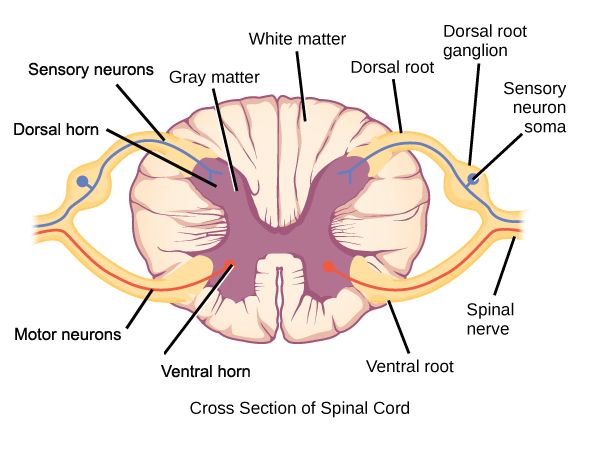
\includegraphics[scale=1.0]{seccion_medula}
  \caption{Sección transversal de médula espinal\cite{seccion_medula}.}\label{fig:seccion_medula}
\end{figure}


\section{Lesiones medulares}
Tras haber tratado los detalles pertinentes de la médula espinal, se procede a estudiar en este apartado el tipo de lesiones que esta puede sufrir y su clasificación según las consecuencias que producen en el paciente.

Una lesión en la médula espinal es cualquier tipo de alteración o anomalía que reduce o interrumpe la transmisión de impulsos nerviosos sensoriales y motrices con el cerebro por debajo del nivel en el que se produce dicha alteración\cite{sci_clasificacion}. Las causas más comunes de este tipo de lesiones son accidentes de tráfico, caídas, actos de violencia o agresiones, accidentes en deportes y actividades de recreación y enfermedades como cáncer, artritis y osteoporosis\cite{causas_sci}. Este tipo de lesiones no solamente producen pérdida de sensibilidad y movilidad sino que suponen una limitación considerable a la hora de realizar tareas esenciales en la vida diaria como vestirse, comer o asearse. Para un paciente con la médula espinal dañada, estas tareas pueden suponer en algunos casos una dificultad inconcebible requiriendo de asistencia externa.
\\
\\
No todas las lesiones de médula espinal son iguales ni suponen las mismas limitaciones, por lo que se va a proceder a la clasificación de las mismas así como los grados de independencia funcional en la realización de tareas esenciales en la vida diaria.


\subsection{Clasificación de lesiones medulares}\label{clasificacion_lesiones}
Para clasificar los tipos de daños en la médula espinal se deben examinar los dermatomas y miotomas para así poder determinar qué partes de la médula están afectadas. Pero antes de proceder a dicha clasificación se van a explicar ciertos términos para comprender mejor los tipos de lesiones en la médula espinal\cite{sci_clasificacion}:

\begin{itemize}
\item[•] \textbf{Tetraplejia:} Se refiere a la pérdida de funciones sensorial y/o motora en la zona cervical de la médula espinal. Afecta a brazos, tronco, piernas y órganos pélvicos.
\item[•] \textbf{Paraplejia:} Implica la pérdida de funciones sensorial y/o motora en las zonas torácica, lumbar o sacral. Se ven afectados tronco, piernas y órganos pélvicos.
\item[•] \textbf{Lesión incompleta:} Se conservan parcialmente las funciones sensoriales y/o motoras por debajo del nivel de la lesión.
\item[•] \textbf{Lesión completa:} Se produce cuando hay una pérdida total de funciones motora y sensoriales en el último segmento sacral de la médula.
\item[•] \textbf{Zona de preservación parcial:} Se refiere a todos aquellos dermatomas y miotomas que están parcialmente conectados a la médula.
\end{itemize}

Las lesiones de médula espinal se pueden clasificar según el estándar creado por la American Spinal Injury Association (ASIA)\cite{ASIA} y que se denomina como International Standards for Neurological and Functional Classification of Spinal Cord Injury. Para clasificar los daños en la médula espinal según este estándar, es necesario realizar un examen neurológico con dos componentes principales: sensorial y motriz. Además, cada componente tiene pruebas esenciales y opcionales que deben realizarse en el paciente. Los elementos esenciales generan una puntuación para determinar la clasificación de los daños en la médula mientras que los opcionales amplían la descripción clínica del paciente\cite{sci_clasificacion}.
\\
\\
El componente esencial del examen sensorial implica probar puntos clave de todos los dermatomas en ambos lados del cuerpo y que se pueden apreciar en la figura \ref{fig:dermatomas_clave}. En cada uno de estos puntos clave se examina la sensibilidad al toque ligero y a una sensación punzante. Se puntúa entonces la respuesta del paciente con un cero si no siente nada, uno si hay una apreciación ligera al estímulo y dos si la respuesta es normal. El componente opcional requiere un estímulo de presión o incluso dolor en cada punto clave de los dermatomas.\\

\begin{figure}[!htb]
\centering
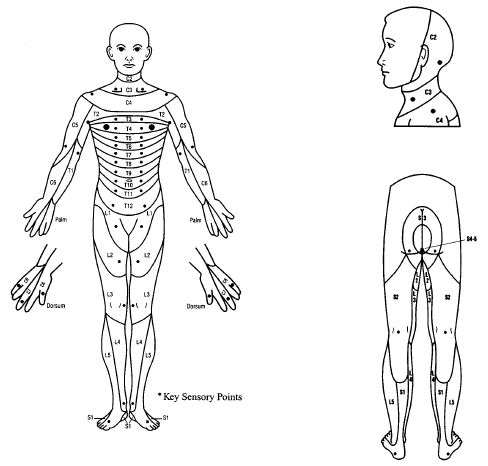
\includegraphics[scale=0.8]{dermatomas_clave}
  \caption{Puntos clave de cada dermatoma para su examen sensorial\cite{dermatomas_puntos}.}\label{fig:dermatomas_clave}
\end{figure}

En cuanto al examen motriz, su componente esencial implica probar un músculo clave de cada miotoma en ambos lados del cuerpo. Algunos de estos músculos son bíceps (flexión de codo) y tríceps (extensión de codo) para la sección cervical, abductores de dedos para la sección torácica, flexión de cadera para la sección lumbar y plantaflexores de tobillos para la sección sacral. Se mide a continuación la fuerza de dichos músculos generando cada uno de ellos una puntuación. Si no hay respuesta alguna del músculo, será puntuado con un cero. En cambio, si hay contracción visible pero sin movimiento la puntuación será de uno. Se valora con un dos un movimiento activo del músculo sin la acción de la gravedad y con un tres si es capaz de moverse en contra de ésta última. Por último, la puntuación será de cuatro si el músculo es capaz de moverse contra una resistencia moderada y de cinco si el movimiento es normal. El componente opcional de este examen implica probar músculos diferentes a los del componente esencial.
\\
\\
Una vez realizados los exámenes sensorial y motriz, se puede determinar el grado de la lesión que sufre la médula espinal. Éste caerá dentro de una de los puntos de la siguiente escala generada por el estándar de la ASIA mencionado previamente:

\begin{itemize}
\item[•] \textbf{Categoría A:} Lesión completa en los segmentos sacrales cuarto y quinto.
\item[•] \textbf{Categoría B:} Lesión incompleta con pérdida sensorial pero no motriz en los segmentos sacrales cuarto y quinto.
\item[•] \textbf{Categoría C:} Lesión incompleta en la que se preserva la función motriz. Además, por debajo del nivel de la lesión, más de la mitad de los músculos clave tienen una puntuación de menos de tres según el examen motriz mencionado previamente.
\item[•] \textbf{Categoría D:} Lesión incompleta en la que se preserva la función motriz. Además, por debajo del nivel de la lesión, más de la mitad de los músculos clave tienen una puntuación de tres o más según el examen motriz mencionado previamente.
\item[•] \textbf{Categoría E:} Funciones sensoriales y motrices normales.
\end{itemize}

Se recoge en la figura \ref{fig:estandar_asia} el estándar generado por la ASIA para la clasificación de lesiones en la médula espinal.\\

\begin{figure}[!htb]
\centering
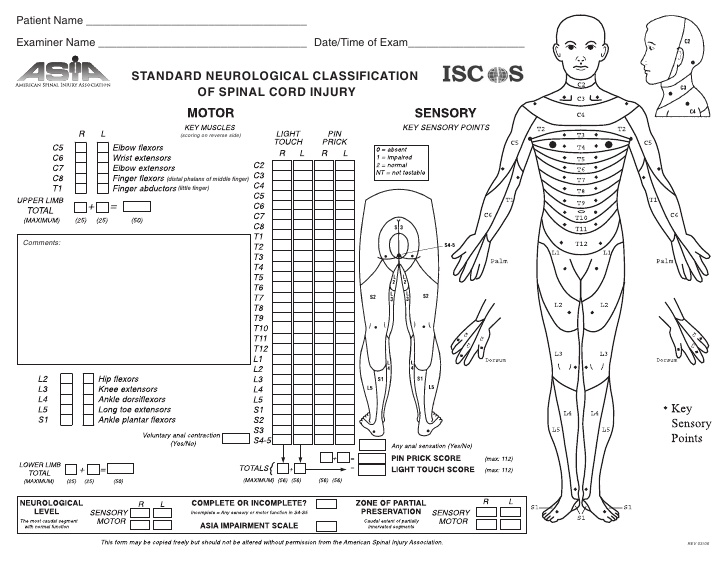
\includegraphics[scale=0.7]{estandar_asia}
  \caption{Plantilla del estándar para clasificación de lesiones en médula espinal\cite{estandar_asia}.}\label{fig:estandar_asia}
\end{figure}

\subsection{Clasificación de independencia funcional}
Además de la clasificación de lesiones de médula espinal, existe la Functional Independence Measure (FIM)\cite{sci_clasificacion} que sirve para determinar el grado de independencia funcional del paciente en la realización de diferentes tareas de la vida diaria. Este estándar se centra en seis áreas: cuidado personal, control de esfínter, movilidad, locomoción, comunicación e interacción social. Dentro de cada área, se evalúan dos o más actividades con un total de 18, como por ejemplo comer, asearse, bañarse o ducharse, vestirse la parte superior o inferior del cuerpo e ir al servicio. Cada tarea se evalúa según la siguiente escala diferenciando si el paciente es independiente o depende de supervisión o asistencia:

\begin{itemize}
\item[•] \textbf{7 puntos - Independencia completa:} La actividad es realizada de forma segura dentro de un tiempo razonable sin ningún tipo de ayuda.
\item[•] \textbf{6 puntos - Independencia modificada:} La actividad requiere la asistencia de algún dispositivo y/o no es realizada dentro de un tiempo razonable y/o no es llevada a cabo de forma segura.
\item[•] \textbf{5 puntos - Supervisión o uso de instalación:} No se requiere asistencia humana pero sí supervisión o algún tipo de soporte o instalación para facilitar la tarea.
\item[•] \textbf{4 puntos - Asistencia mínima:} El sujeto realiza el 75\% o más del esfuerzo requerido para la tarea. 
\item[•] \textbf{3 puntos - Asistencia humana moderada:} El sujeto realiza entre el 50\% y 75\% del esfuerzo requerido para la tarea.
\item[•] \textbf{2 puntos - asistencia máxima:} El sujeto realiza entre el 25\% y 50\% del esfuerzo requerido para la tarea.
\item[•] \textbf{1 punto - Asistencia total:} El sujeto realiza entre el 0\% y 25\% del esfuerzo requerido para la tarea.
\end{itemize}

Por lo tanto, la puntuación total del examen FIM (suma de la puntuación de cada tarea) estima el grado de discapacidad en términos de seguridad y dependencia humana o de algún dispositivo. Con este examen se determina con exactitud qué áreas y tareas de la vida diaria están más afectadas a causa de la lesión en la médula espinal. 


%Se aprecia en la figura \ref{fig:examen_fim} la plantilla para la realización del examen FIM.

%\begin{figure}[!htb]
%\centering
%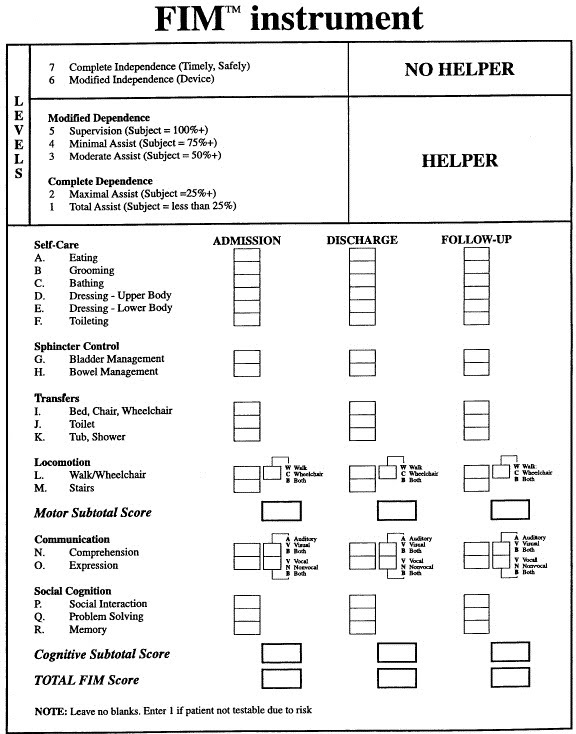
\includegraphics[scale=0.5]{examen_fim}
%  \caption{Plantilla del estándar para clasificación de %independencia funcional\cite{examen_fim}.}\label{fig:examen_fim}
%\end{figure}


\section{Rehabilitación de lesiones en el sistema nervioso central}
A pesar de la gravedad e impacto fisiológico y psicológico que supone una lesión en el sistema nervioso central ya sea procedente de ictus o daño medular, es importante tener en cuenta que sus efectos pueden mitigarse enormemente si se lleva a cabo un proceso adecuado de rehabilitación.
\\
\\
La rehabilitación de este tipo de lesiones entra en el marco de la terapia ocupacional, un tratamiento especializado que ayuda a los pacientes a incrementar su independencia en numerosos aspectos de su vida. Esta terapia permite desarrollar a los pacientes las habilidades necesarias del día a día y así conseguir un nivel de vida satisfactorio e independiente. La terapia ocupacional en el ámbito de la rehabilitación de lesiones en el sistema nervioso central se basa en la adaptación social del paciente y recuperación de habilidades. De forma adicional, se trata de alcanzar ciertos objetivos individuales que son específicos de cada paciente\cite{rehabilitacion}.
\\
\\
Un paciente que sufre una lesión en la médula espinal puede mostrarse desanimado con su terapia cuando sus logros son pocos y distantes en el tiempo. Es por esto por lo que es bueno realizar una gran variedad de actividades adaptadas a cada paciente. De este modo, se impulsa su autoestima resaltando las habilidades funcionales que posee y ya sean físicas, sociales, emocionales, sensoriales o cognitivas. Por lo tanto, la contribución de la terapia ocupacional al rendimiento de los pacientes reside en la realización de actividades útiles para promover su salud física, psicológica e incrementar su independencia funcional.
\\
\\
Es importante que la terapia ocupacional comience lo antes posible tras la estabilización del paciente después de sufrir la lesión. De esta forma, se pueden trabajar con de forma efectiva los siguientes puntos:

\begin{itemize}
\item[•] Evaluar las habilidades y rendimiento del paciente en su hogar, trabajo y tiempo libre.
\item[•] Proporcionar terapia individual para desarrollar actividades de la vida diaria mediante diferentes técnicas.
\item[•] Facilitar técnicas que ayuden al paciente a salvar los efectos de la lesión.
\item[•] Implementar ejercicios y rutinas que ayuden a fortalecer los músculos que hayan podido ser afectados por la lesión.
\item[•] Determinar el tipo de dispositivos de asistencia para otorgar al paciente más independencia en la realización de tareas.
\end{itemize}


Para una correcta realización de la terapia, ésta debe llevarse a cabo en centros especializados con un equipo interdisciplinar de profesionales y un seguimiento riguroso del estado del paciente.
\\
\\
El proceso de rehabilitación se compone tradicionalmente por tres fases: aguda, sentada y sub-aguda. En la fase aguda se efectúan actividades fisioterapéuticas tanto por encima como por debajo del nivel de la lesión para evitar atrofia y mantener en forma los músculos así como un movimiento natural en las articulaciones. Tras esta fase, comienzan los ejercicios para que el paciente consiga, de forma progresiva, incorporarse sobre la cama y sentarse en ésta evitando así reacciones neurovegetativas como consecuencia de la lesión. Por último, comienza la fase sub-aguda en la que se realizan todo tipo de actividades terapéuticas dependiendo del tipo de lesión y de las características del paciente (edad, peso, motivación etc.) De este modo, se incrementan la independencia y habilidades funcionales ya descritas con anterioridad. Hay que tener en cuenta que cada paciente le dará una importancia relativa a cada actividad de modo que éstas se adaptan en consecuencia\cite{tesis_antonio}\cite{etapas_rehabilitacion}.


\subsection{Neuro-rehabilitación de la marcha patológica}
La habilidad del ser humano para caminar está integrada en el sistema nervioso central siendo su principal componente el conjunto de conexiones interneuronales inherentes a la médula espinal. Dichas conexiones se denominan Generadores Centrales de Patrones (GCP) ya que generan el patrón adecuado de activación de los músculos involucrados para caminar. Estos patrones dependen de determinadas entradas sensoriales como la visión y los sistemas vestibular (sentido de movimiento y equilibrio) y propioceptivo (percepción de posición y movimiento del cuerpo) Por lo tanto, el propósito de la tarea que implica caminar es esculpir los patrones de activación de músculos, controlar la transición entre fases del paso y reforzar los resultados satisfactorios\cite{rehabilitacion_caminar}.
\\
\\
Un correcto funcionamiento del sistema nervioso central a la hora de activar los músculos correctamente tal y como se ha mencionado con anterioridad, resulta en la marcha del ser humano. Se trata de un proceso de locomoción en el que el cuerpo se mueve hacia adelante soportando su peso de forma alternativa por ambas piernas. Puesto que es un proceso repetitivo, se puede explicar mediante el ciclo de la marcha recogido en la figura \ref{fig:ciclo_marcha}. El ciclo comienza en el momento en que uno de los pies entra en contacto con el suelo mediante el talón. De este modo, comienza la fase de apoyo que se divide a su vez en dos sub-fases: asimilación del peso y apoyo sobre un miembro. La primera se encarga de estabilizar el miembro absorbiendo el golpe y conservar la inercia del cuerpo mientras que la segunda ofrece un punto de apoyo y estabilidad al cuerpo mientras avanza. Para terminar el ciclo, se entra en la fase de balanceo que comienza con la transición entre la fase anterior y actual levantando el pie del suelo. A continuación, las sub-fases de balanceo inicial, medio y terminal describen la trayectoria de la pierna hasta que vuelve a apoyarse en el suelo y pone fin a una repetición del ciclo de marcha\cite{ciclo_marcha}.\\

\begin{figure}[!htb]
\centering
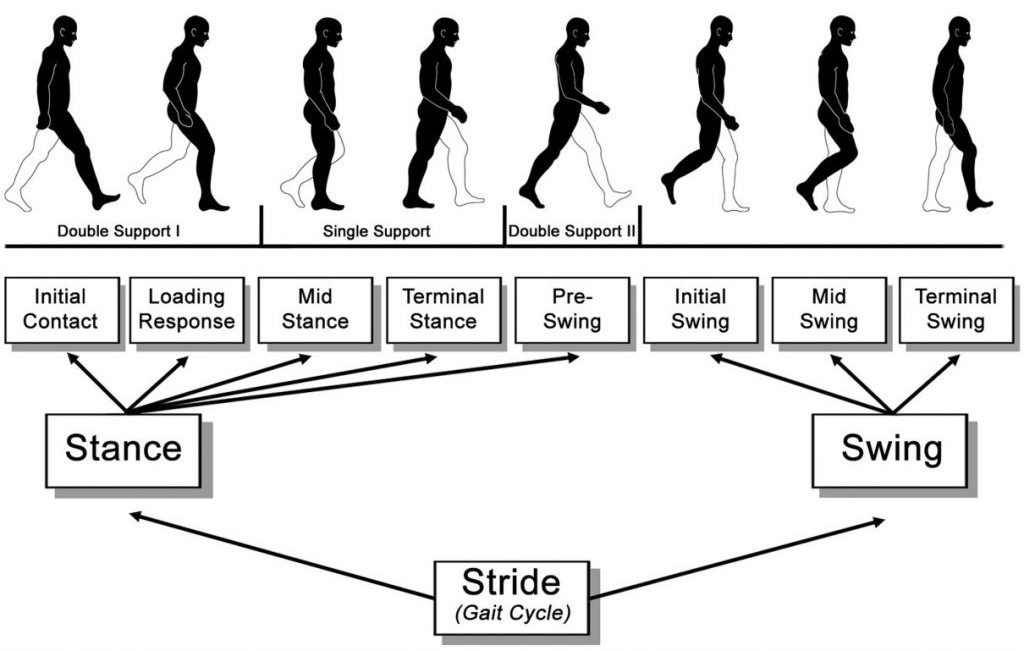
\includegraphics[scale=0.5]{ciclo_marcha}
  \caption{Ciclo de marcha en el ser humano\cite{ciclo_marcha}.}\label{fig:ciclo_marcha}
\end{figure}

Un factor importante en el ciclo de la marcha es la fuerza muscular, pues entrenarla conduce a hipertrofia y una mejor coordinación entre músculos. Sin embargo, incrementar la fuerza muscular no implica mejorar la locomoción y viceversa\cite{recovery_locomotion}. 
\\
\\
Por tanto, la neuro-rehabilitación de la marcha patológica está enfocada a mejorar las habilidades de locomoción del paciente haciendo énfasis en los músculos por debajo del nivel de la lesión. De este modo, las zonas de la médula espinal encargadas de la locomoción pueden ser activadas proporcionando los estímulos adecuados. Esto es posible en el caso de lesiones incompletas ya que para las lesiones completas no se habla de neuro-rehabilitación sino de compensación. En este caso, se pretende conseguir el reaprendizaje de funciones motrices con la ayuda de dispositivos externos. El resultado dependerá de la presencia de circuitos interneruonales capaces de generar patrones de movimiento\cite{recovery_locomotion}.

\subsection{Tecnologías para la neuro-rehabilitación de la marcha patológica}
El proceso de neuro-rehabilitación de la marcha patológica es llevado a cabo por profesionales encargados de ejercitar a los pacientes. Aunque el movimiento en las articulaciones y demás ejercicios es natural y controlado por el terapeuta, se puede perder la consistencia tras largas sesiones y son necesarios varios terapeutas debido al cansancio acumulado, lo cual afecta a la terapia. Por lo tanto, junto a estos métodos de neuro-rehabilitación tradicionales y que son insustituibles, se tienen tecnologías adicionales que favorecen la terapia: entrenamiento robótico del paso y electroestimulación, tecnologías utilizadas en el desarrollo de la prótesis híbrida y en el que está centrado el presente trabajo fin de máster. Se expone a continuación la relación de estas tecnologías con la neuro-rehabilitación de lesiones medulares e ictus dirigida a la marcha patológica.

\subsubsection{Asistencia robótica}

La robótica supone una herramienta de gran valor en la neuro-rehabilitación gracias al uso de exoesqueletos robóticos que pueden definirse como \textit{dispositivos electromecánicos desarrollados para la aumentación de las capacidades físicas del portador o como dispositivo ortopédico para la neuro-rehabilitación de la locomoción o ciclo de marcha}\cite{exoesqueletos}. 
\\
\\
Existen dos tipos principales de exoesqueletos: rígidos y flexibles. El primer tipo, como su nombre indica, implica la utilización de elementos y materiales rígidos para la estructura y fijación del exoesqueleto al paciente. En el segundo caso, se utilizan materiales no rígidos como pueden ser diferentes tipos de textiles. La principal desventaja de un exoesqueleto flexible reside en su alcance en el sentido de su limitada capacidad de aportar fuerza, par y velocidad sobre los miembros del paciente. Esto es una consecuencia inherente al uso de materiales flexibles. Por lo tanto, se usan principalmente cuando se requieren bajos niveles de asistencia o cuando el paciente no tiene dañados los huesos o las articulaciones. Por otra parte, los exoesqueletos rígidos son capaces de proporcionar mayor fuerza, par y velocidad además de hacerlo de forma más precisa para producir movimiento incluso en los casos de parálisis extrema en el paciente. En cuanto a los materiales utilizados, se desea un equilibrio entre integridad estructural y peso de modo que se emplea acero, aluminio, fibra de carbono o piezas impresas en 3D con filamentos de polímeros termoplásticos acrilonitrilo butadieno estireno (ABS) y ácido poliláctico (PLA).\cite{estudio_exoesqueletos}\cite{comparacion_exoesqueletos}. Se pueden apreciar ejemplos de ambos tipos de exoesqueletos en la figuras \ref{fig:exoesqueleto_rigido} y \ref{fig:exoesqueleto_flexible}.\\

\begin{figure}[!htb]
\minipage{0.35\textwidth}

  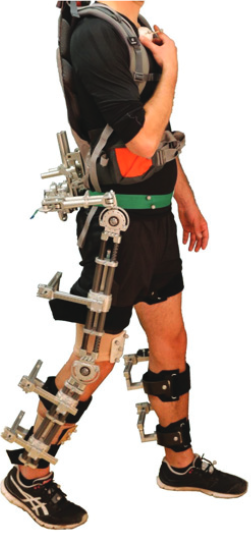
\includegraphics[width=\linewidth]{exoesqueleto_rigido}
  \caption{Exoesqueleto rígido para neuro-rehabilitación de marcha patológica\cite{exoesqueleto_rigido}}\label{fig:exoesqueleto_rigido}
\endminipage\hfill
\minipage{0.55\textwidth}%
  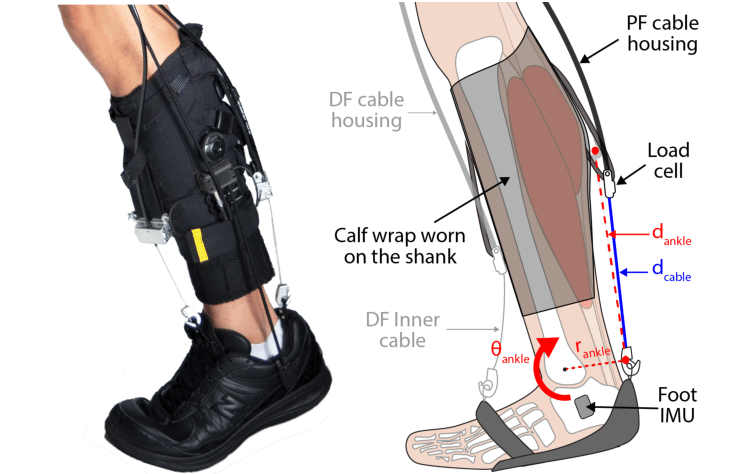
\includegraphics[width=\linewidth]{exoesqueleto_flexible}
  \caption{Exoesqueleto flexible para el control del movimiento del tobillo\cite{exoesqueleto_flexible}}\label{fig:exoesqueleto_flexible}
\endminipage

\end{figure}

Los exoesqueletos disponen de diferentes tipos de actuadores para generar movimiento. Se describen a continuación algunos de los más comunes y que además forman parte del exoesqueleto utilizado en la prótesis híbrida\cite{estudio_exoesqueletos}\cite{tesis_antonio}\cite{actuadores_exoesqueletos}:

\begin{itemize}
\item[•]\textbf{Motores de corriente continua:} Es el tipo de actuador más usado en exoesqueletos ya que es fácil de controlar y ofrece respuestas rápidas y un par elevado para manejar las partes más pesadas del exoesqueleto. Según la aplicación y el tipo de control requerido se usan estos motores de forma directa o con una reductora si lo que se pretende es un movimiento rápido y fuerte o lento y controlado, respectivamente. Además, se usan motores con escobillas si se desea prescindir de electrónica o bien motores sin escobillas si lo que se desea es un mejor ratio potencia/peso.

\item[•]\textbf{Almacenamiento de energía elástica:} Se trata de todo tipo de dispositivo, como resortes o muelles, capaz de almacenar energía elástica durante determinadas fases del ciclo de marcha para liberarla después en otras fases. Es un método robusto y que no requiere de fuentes de energía pero no se puede tener un control preciso sobre la respuesta que ofrecen estos actuadores.

\item[•]\textbf{Accionamientos hidráulicos:} Es el actuador con el mejor ratio par/peso ya que puede generar valores muy elevados de fuerza. Esto se debe a la inyección de un fluido a alta presión, como puede ser aceite, dentro de un cilindro para producir movimiento en un émbolo sujeto a la prótesis. Sin embargo, su principal desventaja implica la necesidad de una bomba junto a un depósito de aceite lo que supone problemas de ruido y fugas además de un control no lineal del movimiento.

\item[•]\textbf{Accionamientos neumáticos:} Al igual que los actuadores hidráulicos, poseen un gran ratio fuerza/peso, en este caso debido a la inyección de aire a alta presión del mismo modo que en el actuador anterior. Aunque es más ligero que éste y produce movimientos más naturales acorde a un comportamiento muscular normal, también sufre problemas de fugas, ruido y movimiento no lineal.




%\item[•]\textbf{Motores ultrasónicos:} Su funcionamiento se basa en el fenómeno piezoeléctrico, es decir, el estator recibe energía eléctrica y la tranforma en vibraciones mecánicas que pasan al rotor, elemento que transforma esas vibraciones en movimiento circular mediante fricción. Esto es posible debido a los materiales piezoeléctricos que conectan estator y rotor. su principal ventaja es que pueden llegar a tener un ratio par/volumen hasta 20 veces superior al de los motores de corriente continua. Además de ser ligero y compacto, no produce ruido y puede operar a muy baja velocidad con gran precisión. Sin embargo, son muy difíciles de fabricar y por lo tanto una carga económica importante.

%\item[•]\textbf{Aleaciones de memoria de forma:} Son aleaciones metálicas, principalmente de cobre, aluminio y níquel que, ante una deformación plástica, son capaces de recuperar su forma anterior a ésta si alcanzan cierta temperatura debido a cambios en la estructura cristalina de la aleación. Estos actuadores pueden proporcionar grandes fuerzas y desplazamientos con un buen ratio potencia/peso. Sin embargo, se debe tener en cuenta que su actuación no es simétrica ya que los movimientos de contracción son generalmente más rápidos que los de elongación, lo que dificulta su control.


%\item[•]\textbf{Polímeros electroactivos:} Es un tipo de material elástico desarrollado recientemente y cuyas características son muy similares a las del músculo humano. El movimiento en este tipo de material se produce al ser estimulado con campos eléctricos. Presenta un alto rango de potencia además de una conversión de energía eléctrica a mecánica altamente eficiente. Sin embargo, tiene un ratio par/peso reducido por lo que de momento no es un material óptimo para exoesqueletos de modo que es necesaria más investigación para mejorar sus propiedades.
\end{itemize}


Teniendo en cuenta las características y capacidades de los exoesqueletos, si se emplean como herramientas de neuro-rehabilitación, es posible replicar los ejercicios que el terapeuta efectúa sobre el paciente con diferentes configuraciones de fuerza, par y velocidad. Además, se pueden llevar a cabo ejercicios que son imposibles para un terapeuta debido a limitaciones de fuerza, repetibilidad o sensibilidad\cite{robotica_rehabilitacion}.
\\
\\
Debido a la utilidad y versatilidad del uso de la robótica en forma de exoesqueleto en la neuro-rehabilitación, surge el concepto de assist-as-needed (AAN)\cite{assist_as_need} y que implica la asistencia y corrección de los movimientos del paciente. De este modo, el paciente trata de efectuar un ejercicio mientras que el robot le proporciona asistencia solamente cuando la necesita. El nivel de asistencia varía en función de la desviación del paciente respecto a la trayectoria planteada por el ejercicio por lo que un exoesqueleto robótico tiene en este campo un gran alcance ya que puede administrar varios patrones motrices y sensoriales. El hecho de aportar esta variabilidad motriz y sensorial potencia la habilidad de aprendizaje de la médula espinal evitando las incongruencias procedentes de un patrón fijo de movimientos para caminar.
\\
\\
Una de las ventajas del uso de exoesqueletos en neuro-rehabilitación de marcha patológica es su mayor seguridad y control sobre el ejercicio respecto a la terapia tradicional. Además, no solo permiten rehabilitar el ciclo de marcha sino que potencian las capacidades físicas del paciente si se sigue usando esta herramienta mucho después del momento en que se produjo la lesión. Es importante considerar también el factor de motivación del paciente puesto que un exoesqueleto ayuda a conseguir resultados de forma más rápida y efectiva mejorando así la velocidad y eficiencia de la neuro-rehabilitación. Por otra parte, es importante considerar que dos tercios de los pacientes con lesiones medulares sufren de sobrepeso u obesidad debido a la falta de ejercicio físico. En este aspecto, un exoesqueleto ayuda a combatir el sobrepeso ya que reduce el tiempo requerido para realizar los ejercicios de neuro-rehabilitación, aumenta la cantidad de actividad física realizada por el paciente y ayuda a mejorar la composición de determinadas partes del cuerpo. Sin embargo, la mayoría de los exoesqueletos disponibles son capaces de soportar pacientes de hasta 100 Kg lo que deja fuera de esta terapia a un número considerable de sujetos\cite{ventajas_desventajas_exoesqueletos}. 
\\
\\
Por último, desde un punto de vista más técnico, clínico y económico, un exoesqueleto está formado por una estructura compuesta de diferentes tipos de materiales como acero, aluminio, fibra de carbono, textiles adecuados así como actuadores ya descritos. Esto supone un conjunto de elementos no asequible para cualquier individuo o institución. Además, se trata de una herramienta generalmente aparatosa y/o pesada por lo que su uso queda principalmente reducido a un ambiente clínico y no a la vida diaria del paciente en su hogar, trabajo u otras áreas.
\\
\\
Para terminar, uno de los dispositivos más utilizados en la neuro-rehabilitación del ciclo de marcha en ambientes clínicos es el Lokomat\cite{lokomat}. Está formado por una prótesis robótica especializada para caminar junto a un sistema de soporte del peso corporal y una cinta. Dispone de 4 grados de libertad mediante movimientos lineales: articulaciones derecha e izquierda de cadera y rodillas. Las piernas del paciente están sujetas por la prótesis y lo movimientos lineales de la misma sincronizados con la velocidad de la cinta de caminar. El concepto de AAN entra en juego en el Lokomat permitiendo al paciente moverse libremente dentro de un espacio designado para el patrón del paso. Se consigue por tanto más variabilidad y libertad de movimiento y adaptación del paso para cada paciente que siguiendo la neuro-rehabilitación tradicional. Se muestra en la figura \ref{fig:lokomat} el dispositivo descrito.\\

\begin{figure}[!htb]
\centering
\minipage{0.6\textwidth}
  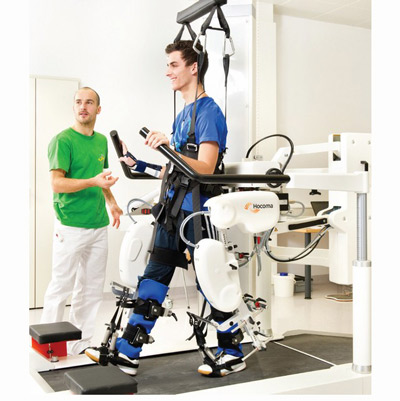
\includegraphics[width=\linewidth]{lokomat}
  \caption{Dispositivo Lokomat para neuro-rehabilitación de la marcha patológica\cite{lokomat_imagen}.}\label{fig:lokomat}
\endminipage\hfill
\end{figure}

\subsubsection{Asistencia por electroestimulación mediante neuroprótesis}

Una alternativa para trabajar sobre los músculos del paciente es la electroestimulación o estimulación eléctrica de los tejidos neuromusculares. Con una configuración adecuada se pueden estimular músculos paralizados tras la lesión medular para permitir caminar al paciente y llevar a cabo la neuro-rehabilitación\cite{electroestimulacion2}.
\\
\\
Es preciso diferenciar entre electroestimulación muscular, del inglés Muscle Electrical Stimulation (MES) o simplemente electroestimulación y electroestimulación funcional, es decir Functional Electrical Stimulation (FES). La primera implica la tranmisión de pulsos eléctricos a los músculos para conseguir su estimulación en forma de contracción muscular con diferentes fines como puede ser el entrenamiento deportivo\cite{sanitas}. La segunda consigue emparejar la estimulación de forma simultánea o intermitente con una determinada tarea o ejercicio, por ejemplo, caminar o realizar ciertos movimientos con las extremidades. Esto consitutuye una neuroprótesis motora o NeuroProsthesis (NP)\cite{tesis_antonio}.
\\
\\
En su forma más básica, la electroestimulación es la interacción mediante señales eléctricas con partes del cuerpo que conservan respuesta a dicho estímulo. De este modo, aplicando pequeños pulsos eléctricos sobre músculos o nervios se puede producir su contracción y por lo tanto estimulación y movimiento artificial en el cuerpo. Sin embargo, el resultado final depende de cada patología y caso del paciente así como la efectividad con la que se lleva a cabo la electroestimulación y que involucra el tipo de electrodos utilizados, su colocación, selectividad de músculos, impedancia de la piel, integridad muscular etc. \cite{electroestimulacion}.
\\
\\
Para la aplicación de corriente existen diferentes tipos de electrodos: superficiales (parches sobre la piel), transcutáneos (aguja con un cable por dentro para atravesar la piel y contactar con el músculo o nervio) o implantados (permanentemente fijados a los nervios para largo uso siempre que sea biocompatible en el paciente)\cite{tipos_electrodos}
Una vez seleccionado el tipo de electrodos, se colocan dos por cada músculo o nervio de modo que uno sirve como cátodo y otro como ánodo. Es importante colocar los electrodos correctamente, es decir, sobre puntos motrices de los músculos y nervios, así como conseguir una selectividad adecuada. Éste último término hace referencia a la estimulación de los músculos y nervios deseados con la intensidad adecuada para evitar efectos adversos\cite{limitaciones_fes}. Se aprecia en las figuras \ref{fig:electrodo_superficial} y \ref{fig:electrodo_percutaneo} algunos de los diferentes tipos de electrodos usados en electroestimulación.\\

\begin{figure}[!htb]
\minipage{0.45\textwidth}
  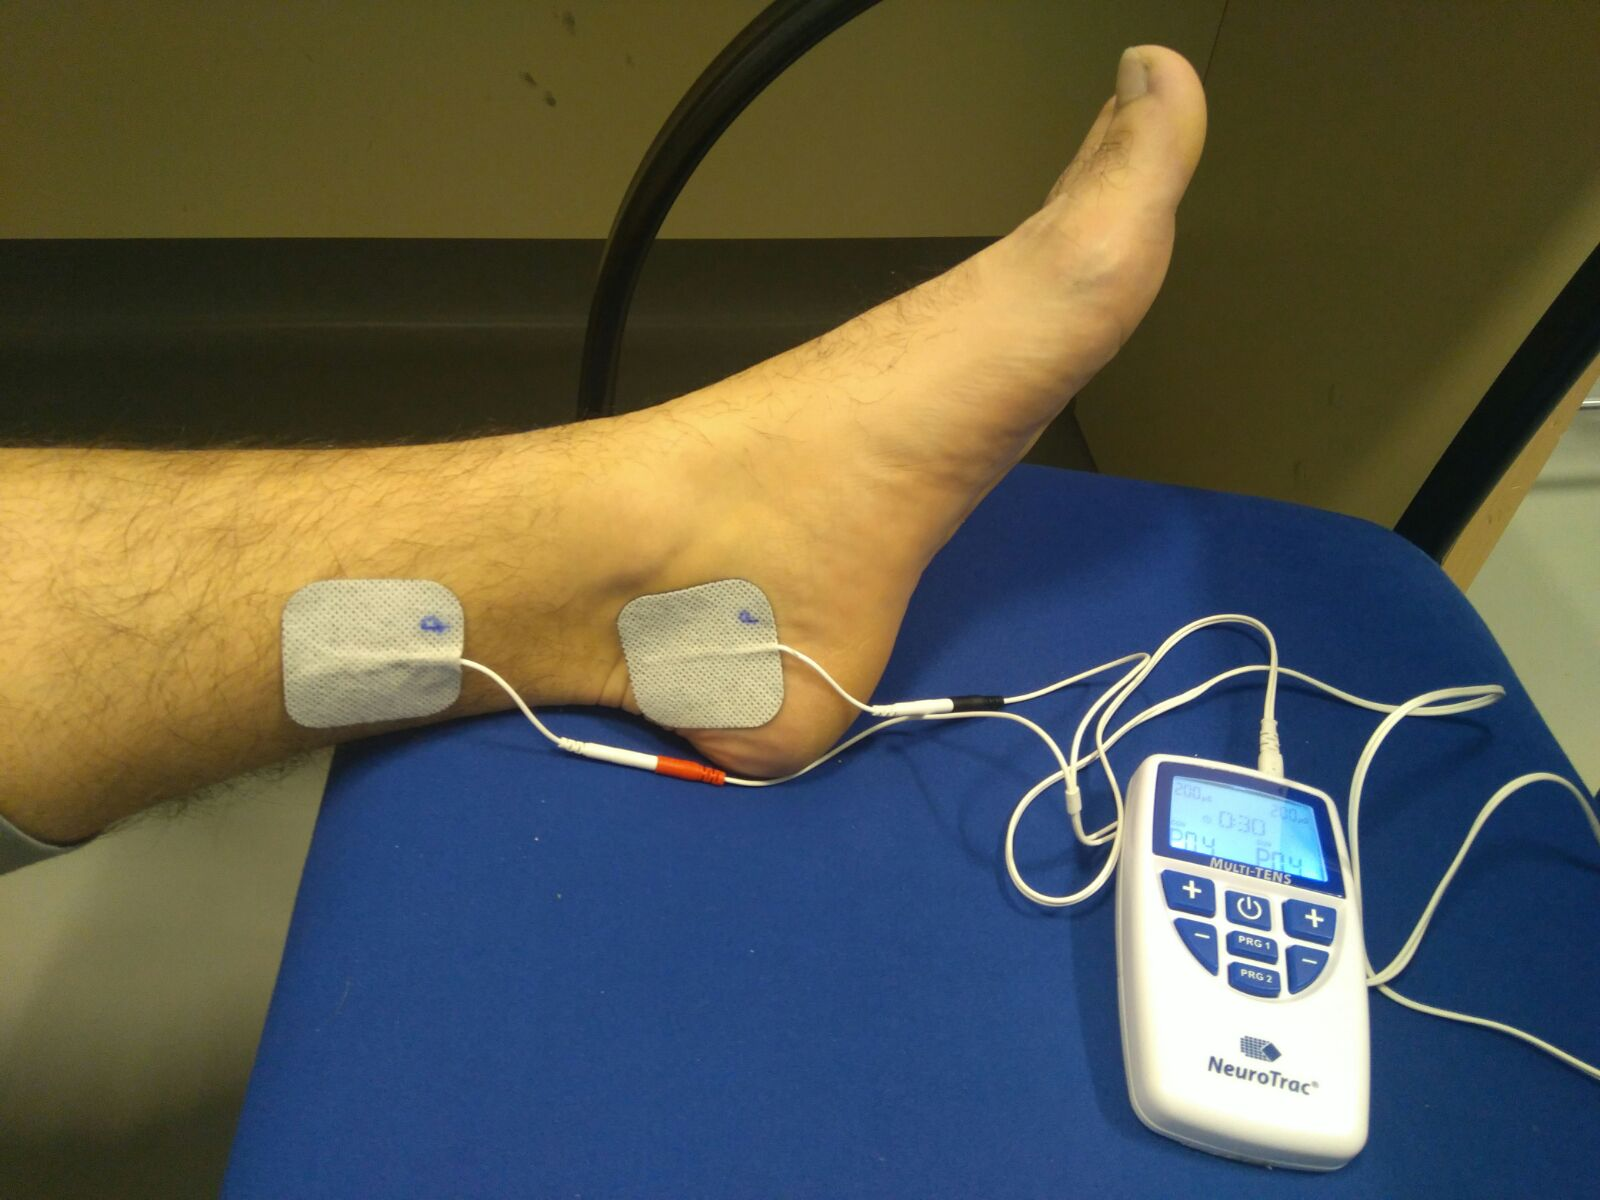
\includegraphics[width=\linewidth]{electrodo_superficial}
  \caption{Electrodo superficial\cite{electrodo_superficial}.}\label{fig:electrodo_superficial}
\endminipage\hfill
\minipage{0.45\textwidth}
  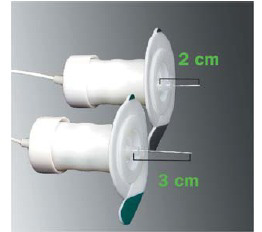
\includegraphics[width=\linewidth]{electrodo_percutaneo}
  \caption{Electrodo percutáneo\cite{electrodo_percutaneo}.}\label{fig:electrodo_percutaneo}
\endminipage\hfill
\end{figure}

La aplicación de estímulos eléctricos puede llevarse a cabo mediante pulsos de tensión o de corriente. Usar pulsos de tensión implica que el daño producido sobre los tejidos del cuerpo viene dado por el valor de densidad de corriente, lo que influye en la respuesta muscular de modo que si existe una alta impedancia entre le electrodo y el músculo, la corriente que llega al mismo para un determinado valor de tensión será menor. Por otro lado, utilizar pulsos de corriente imita mejor los movimientos naturales del cuerpo y muestra resultados más consistentes y repetibles así como menor variación en la impedancia de la piel y otros tejidos. Por lo tanto, una configuración óptima evita que la impedancia varíe a lo largo del proceso y por tanto afecte a la corriente que llega al músculo, cuya respuesta depende directamente de ésta\cite{FES}. Por ello, es preferible utilizar pulsos de corriente en vez de pulsos de tensión y para lo que es necesario utilizar una fuente de corriente adecuada, dispositivo que se explicará más adelante.
\\
\\
Los parámetros de un pulso de corriente son amplitud, ancho de pulso, periodo inter e intra pulso y forma del pulso\cite{parametros_FES}. La forma del pulso determina cómo se va a aplicar corriente entre los electrodos generando diferentes patrones de pulsos de corriente. Algunos de estos patrones se explican a continuación\cite{FES} y pueden apreciarse en la figura \ref{fig:patrones_pulsos}:

\begin{itemize}
\item[•] \textbf{Pulso monofásico:} Se aplica corriente en un solo sentido, es decir, de ánodo a cátodo o de cátodo a ánodo. Produce daño en tejidos y deterioro del electrodo por su efecto polarizante al alterar la distribución iónica de la zona de aplicación.
\item[•] \textbf{Pulso bifásico asimétrico:} Se aplica una corriente en un sentido y después otra diferente en el otro. Al ser bidireccional permite a los iones circular en dos sentidos minimizando la redistribución de éstos y el daño en tejidos y electrodos.
\item[•] \textbf{Pulso bifásico simétrico:} Se aplica corriente primero en un sentido y después ese mismo valor de corriente en el otro. Se consigue neutralizar el efecto polarizante pero la corriente anódica puede suprimir parte de la corriente catódica y viceversa. Por tanto, los pulsos anódicos y catódicos se distancian en el tiempo para evitar el mencionado efecto.
\end{itemize}

\begin{figure}[!htb]
\centering
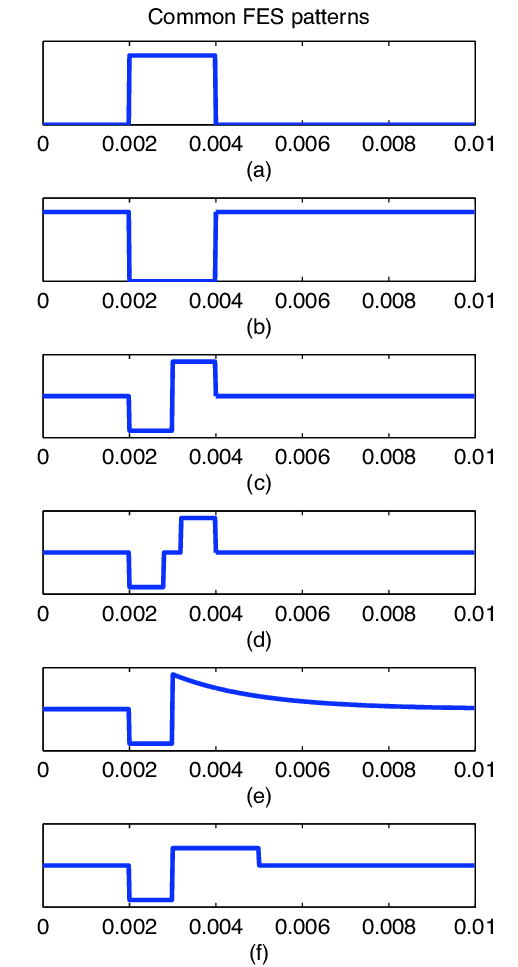
\includegraphics[scale=0.3]{patrones_pulsos}
  \caption{Patrones de pulsos de corriente\cite{FES}. Pulso monofásico (a) y (b), pulso bifásico simétrico sin espaciado (c) y con espaciado temporal (d) y pulsos bifásicos asimétricos (e) y (f). Se aprecia que el pulso (e) tiene una rampa para que la estimulación sea más natural y suave.}\label{fig:patrones_pulsos}
\end{figure}

Una vez expuestos algunos de los posibles patrones de pulsos, la amplitud es la intensidad de corriente ($mA$) aplicada de ánodo a cátodo o de cátodo a ánodo durante el tiempo especificado por el ancho de pulso (del orden de $us$ y $ms$). El periodo intra pulso es el tiempo que separa la aplicación de corriente positiva y negativa en un pulso bifásico. Por último, es necesario indicar que la electroestimulación se efectúa mediante trenes de pulsos, es decir, repeticiones de pulsos hasta conseguir el efecto deseado en los músculos. El periodo de repetición de pulsos está determinado por el periodo inter pulso y según su configuración da lugar a diferentes tipos de trenes de pulsos\cite{tipos_repeticion} mostrados en la figura \ref{fig:tipos_repeticion}:


\begin{itemize}
\item[•] \textbf{Tren de frecuencia constante:} Implica la repetición de un pulso de corriente a frecuencia constante. 
\item[•] \textbf{Tren de frecuencia variable:} Se comienza el tren con dos pulsos próximos en el tiempo y se sigue con una repetición constante de pulsos simples.
\item[•] \textbf{Tren de pulsos dobles:} Se repiten a frecuencia constante dos pulsos próximos en el tiempo. 
\end{itemize}

El motivo por el que se utilizan pulsos dobles es para aprovechar el efecto muscular en forma de un incremento de fuerza considerable ante estímulos de alta frecuencia (dos pulsos de corriente seguidos) Se utiliza de forma limitada porque produce fatiga en el músculo\cite{catch_like}.\\

\begin{figure}[!htb]
\centering
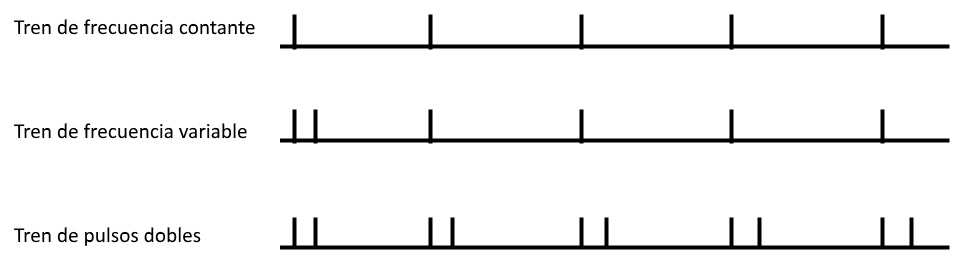
\includegraphics[scale=0.5]{tipos_repeticion}
  \caption{Tipos de trenes de pulsos según su periodo inter pulso. Cada línea vertical indica un pulso de corriente.}\label{fig:tipos_repeticion}
\end{figure}

Se muestra en la figura \ref{fig:tren_pulsos} un tren de pulsos bifásicos asmétricos y sus parámetros ya explicados.\\

\begin{figure}[!htb]
\centering
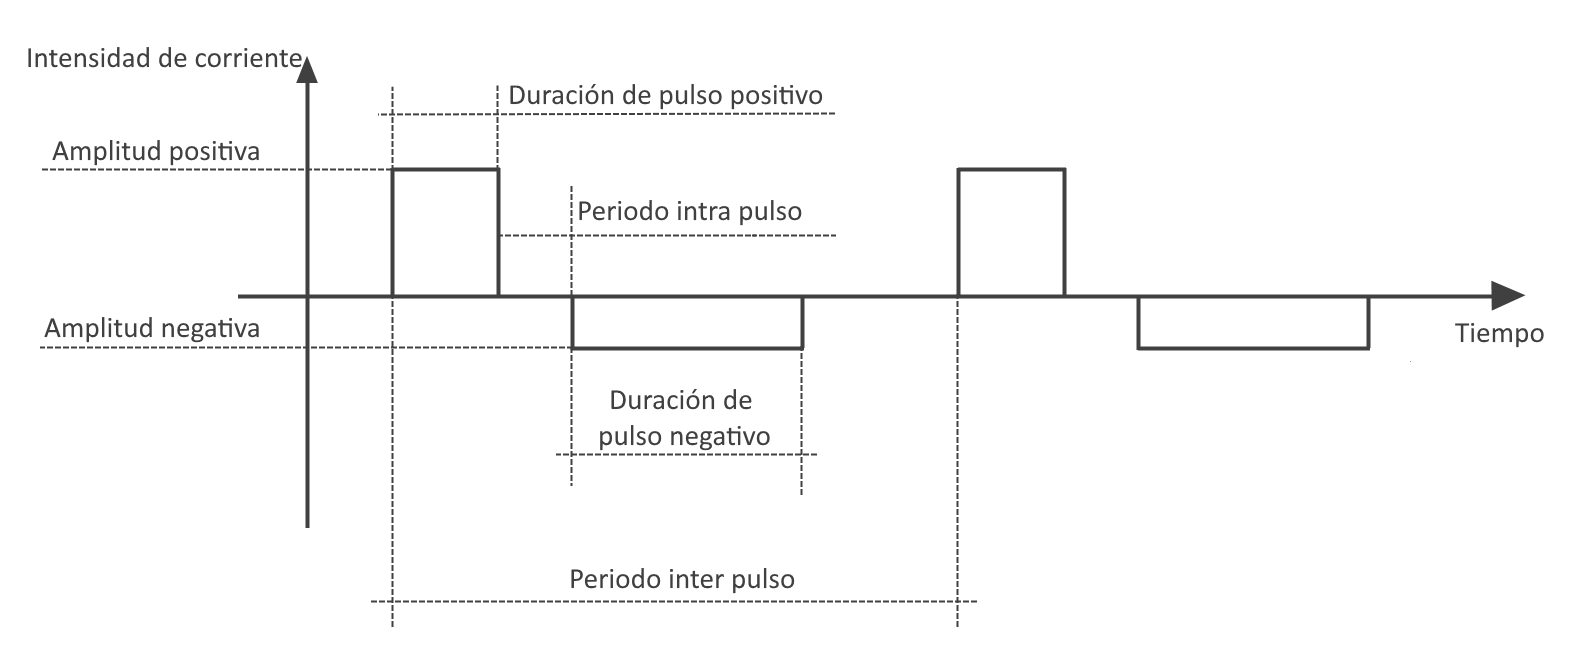
\includegraphics[scale=0.4]{tren_pulsos}
  \caption{Tren de pulsos bifásicos asimétricos.}\label{fig:tren_pulsos}
\end{figure}


El uso de la electroestimulación tiene beneficios como refuerzo de músculos, mejora de la circulación sanguínea, reducción de sensación de dolor y retraso de la atrofia muscular y de la espasticidad\cite{ventajas_FES}. Por otra parte, también existen desventajas como puede ser daño y fatiga muscular y alteraciones en la fuerza y tejidos y fibras musculares\cite{electroestimulacion}. Además, existen limitaciones en la aplicación de esta tecnología para neuro-rehabilitación y que son intrínsecas a la activación de músculos mediante estimulación eléctrica. En primer lugar, la respuesta al estímulo no es lineal y varía con el tiempo. Además, el músculo se va fatigando lo que altera su comportamiento el cual también varía según la resistencia a la fatiga y fuerza muscular. Por último, hay que considerar que hay un retardo considerable entre la generación del estímulo y  la respuesta por parte del músculo\cite{limitaciones_fes}.
\\
\\
Como ejemplo de aplicación de la electroestimulación se tiene el dispositivo comercial de Odstock\cite{estimulador_odstock} que permite corregir el pie caído\cite{pie_caido}. Dispone de un único canal, es decir, una salida por la que transmitir un tren de pulsos mediante el uso de electrodos superficiales sobre el nervio peroneo. Se muestra este dispositivo en la figura \ref{fig:estimulador_odstock}\\

\begin{figure}[!htb]
\centering
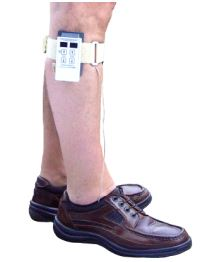
\includegraphics[scale=0.8]{estimulador_odstock}
  \caption{Electroestimulador de Odstock para el pie caído.}\label{fig:estimulador_odstock}
\end{figure}


\subsubsection{Prótesis híbridas}\label{protesis_hibridas}
Se han revisado las tecnologías de electroestimulación muscular y exoesqueletos robóticos para la asistencia en le neuro-rehabilitación de la marcha patológica. Ambas otorgan ventajas únicas pero al mismo tiempo implican ciertas limitaciones. Es por ello por lo que es posible combinar  FES y exoesqueletos robóticos, para potenciar sus ventajas y mitigar sus limitaciones durante la neuro-rehabilitación, la cual es mucho más eficaz en esta configuración de tecnologías que utilizando cualquiera de ellas de forma independiente\cite{protesis_hibridas}.
\\
\\
En primer lugar, se puede hablar de las neuroprótesis híbridas, las cuales combinan la tecnología FES para producir movimiento mediante contracciones musculares con un exoesqueleto pasivo o no motriz. De este modo, toda la actividad motriz proviene de la eslectroestimulación, es decir, de los músculos del paciente, mientras que el exoesqueleto se encarga de aportar estabilidad bloqueando articulaciones cuando sea necesario o asistiendo en determinados movimientos.
\\
\\
Partiendo de la configuración anterior, es posible el uso de la tecnología FES junto a un exoesqueleto motriz para abordar la mayor cantidad de casos en la neuro-rehabilitación de la marcha patológica. Una de las diferentes soluciones existentes implica un control cooperativo de los motores del exoesqueleto y la estimulación muscular. Esto consigue minimizar la contribución del torque ofrecido por el exoesqueleto y así maximizar la fuerza generada por los músculos mediante electroestimulación con parches superficiales\cite{FES_exoesqueleto_motriz}. Por un lado, el control del torque de los motores se consigue con una realimentación de la medida de ángulos de flexión de cadera y rodillas para seguir una trayectoria predefinida. Por otra parte, el control de la estimulación muscular se lleva a cabo mediante una estimación del momento de las articulaciones. Efectivamente, esta configuración ha sido probada en tres sujetos con diferentes niveles de lesión medular y todos ellos han mostrado un ciclo de marcha consistente y repetible con una actuación reducida por parte del exoesqueleto\cite{FES_exoesqueleto_motriz}.
\\
\\
Se considera entonces que existen dos principales tecnologías con el mejor potencial para una neuro-rehabilitación efectiva: FES y exoesqueletos motrices. Además, se ha demostrado que su combinación impulsa los beneficios y resultados más allá del uso individual de una de estas dos técnicas. Sin embargo, se puede dar un paso más y hacer uso de electrodos implantados para la electroestimulación funcional. A diferencia de los electrodos superficiales, un implante produce contracciones musculares más fuertes, consistentes y selectivas que cualquier otra técnica de electroestimulación, incluso para músculos con elevado grado de parálisis. De este modo, se da prioridad a los músculos del sujeto como fuente de movimiento potenciando así las ventajas que conlleva la estimulación eléctrica muscular ya discutidas previamente. Por tanto, el exoesqueleto motriz queda en un segundo plano para asistir al sujeto cuando lo necesite, por ejemplo, cuando sus músculos comiencen a fatigarse o en el caso de desviarse de la trayectoria adecuada. Esta configuración permite la utilización de exoesqueletos más ligeros debido a su papel secundario en la neuro-rehabilitación y de los cuales se puede incluso prescindir en determinadas actividades haciendo uso solamente de la electroestimulación. Se puede apreciar un ejemplo de este tipo de prótesis híbrida en la figura \ref{fig:protesis_hibrida}.\\

\begin{figure}[!htb]
\centering
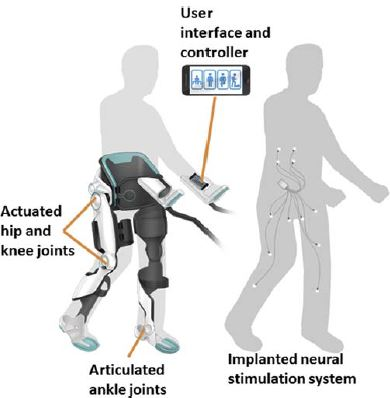
\includegraphics[scale=1.0]{protesis_hibrida}
  \caption{Modelo de prótesis híbrida que combina FES y un exoesqueleto motriz\cite{protesis_hibridas}.}\label{fig:protesis_hibrida}
\end{figure}

A pesar de los progresos realizados en las tecnologías para la neuro-rehabilitación, todavía existen limitaciones tales como la velocidad de la marcha y la comodidad y sencillez para usar diferentes tipos de prótesis. En cuanto al primer problema, se consideran 0.8$m/s$ y 500$m$ como velocidad y distancia promedio aceptables para la deambulación comunitaria\cite{requerimientos_ambulacion_1}\cite{requerimientos_ambulacion_2}, es decir, la realización de tareas básicas en el entorno donde reside el paciente como por ejemplo ir a comprar. Sin embargo, las tecnologías mencionadas no siempre consiguen que el paciente alcance dichos valores quedándose en 0.2-0.4$m/s$ usando solamente electroestimulación\cite{velocidad_FES} y 0.22-0.27$m/s$\cite{velocidad_exoesqueleto_1}\cite{velocidad_exoesqueleto_2} y hasta 170$m$\cite{distancia_exoesqueleto} valiéndose únicamente del exoesqueleto motriz. Pero estos valores dependen en gran medida de cada paciente ya que tanto la velocidad de marcha como la distancia máxima que puede realizar dependen notablemente de la fuerza y resistencia de la mitad superior del cuerpo. Esto se debe a que un exoesqueleto motriz requiere una fuerza considerable por parte de los brazos y el tronco para aportar estabilidad y asistir con la propulsión en la marcha. En cuanto al segundo problema, cualquier tipo de prótesis ya sea híbrida o solamente un exoesqueleto o electroestimulador, requiere ser calibrada antes de utilizarse, colocar los parches sobre la piel correctamente, tener las baterías cargadas en el caso correspondiente etc. Por tanto, es importante que estas preparaciones sean lo más rápidas y sencillas posible para facilitar la neuro-rehabilitación y evitar su abandono.


\subsubsection{Sensores}

Hasta ahora se ha hablado de actuadores como exoesqueletos robóticos y electroestimulación como tecnologías para la neuro-rehabilitación de la marcha patológica. Sin embargo, no se ha mencionado el control de mencionadas herramientas, el cual se va a discutir en este apartado. 
\\
\\
El control de un exoesqueleto, un dispositivo de electroestimulación o cualquier sistema puede realizarse en lazo abierto o en lazo cerrado. El primero de ellos implica el uso de estas herramientas de neuro-rehabilitación configuradas para una tarea determinada sin ningún tipo de información del ambiente, es decir, el paciente que interactúa con ellas. En cambio, si se dispone de información del estado del paciente y/o de la herramienta de neuro-rehabilitación durante la realización del ejercicio para detectar las fases de la marcha, existe mucho más control sobre el proceso así como resultados más satisfactorios y precisos. Para ello, se necesita sensar determinados parámetros de importancia para la correcta realización de los ejercicios de neuro-rehabilitación. Se muestran a continuación algunos de los sensores y medición de parámetros más comunes\cite{sensores}:

\begin{itemize}
\item[•] \textbf{Unidad de Medidas Inerciales:} Tienen gran capacidad de sensar los movimientos del cuerpo mediante acelerómetros y giróscopos cada vez más adaptables al ser humano debido a su reducción de tamaño y peso. En este sentido, se puede obtener información tridimensional midiendo aceleraciones, ángulos y velocidades angulares en los tres ejes espaciales. La principal ventaja de este sensor es que solamente necesita un punto de sujeción sobre el paciente o exoesqueleto.

\item[•] \textbf{Goniómetros:} Se utilizan para medir ángulos entre las dos partes de un miembro unidas por una articulación, por ejemplo, el ángulo entre la tibia y el fémur medido desde la rodilla. Existen goniómetros flexibles y en forma de potenciómetros aunque son muy sensibles debido a que están colocados en una articulación y necesitan dos puntos de sujeción.

\item[•] \textbf{Consumo de corriente en motores:} En el caso de los exoesqueletos, se puede medir el consumo de corriente de sus motores. Esto es útil ya que un motor de corriente continua al que se le restringe el movimiento responderá consumiendo más corriente para vencer esta resistencia. Por lo tanto, se pude tomar como indicativo de que el paciente está ejerciendo fuerza contra el exoesqueleto, es decir, se desvía de la trayectoria prevista. 

\item[•] \textbf{Sensor de fuerza resistivo:} Se utilizan principalmente para medir fuerza y distribución normal de presión en la pisada durante la fase del ciclo de marcha correspondiente. Sin embargo, no son indicados para medir fuerzas de corte o de cizalla. 

\item[•] \textbf{Electromiografía (EMG):} La electromiografía es un procedimiento mediante el cual se puede registrar la actividad eléctrica muscular denominada electromiograma. Esto permite determinar el estado de salud muscular así como el de las neuronas motoras que controlan los músculos esqueléticos\cite{EMG}. En el ámbito de la neuro-rehabilitación, se utiliza para obtener un mayor control sobre el estado de los músculos así como de su nivel de fatiga. Esto permite reforzar el aprendizaje del paciente mediante el ajuste de parámetros en el entrenamiento midiendo la intesidad con la que se activa cada músculo en todo momento\cite{EMG2}. La medición de esta actividad eléctrica se recoge en electrodos superficiales o transcutáneos (una fina aguja fina con el electrodo en forma de cable por dentro) Los primeros son más cómodos y no se descolocan con la actividad física pero arrojan mediciones más imprecisas. Los segundos ofrecen mayor calidad en las mediciones pero pueden ser dolorosos y perder efectividad ante movimientos bruscos, como pueden ser los del ciclo de marcha. Sin embargo, esta técnica no es fácilmente aplicable ya que puede resultar tedioso obtener mediciones correctas, especialmente en pacientes con sobrepeso u obesidad puesto que será más difícil llegar al músculo para medir su actividad.
\end{itemize}

%Una vez analizados algunos de los sensores utilizados en la electroestimulación y exoesqueletos, el tipo de control, objetivos y limitaciones del proceso de neuro-rehabilitación dependerá de cada aplicación así como del paciente. Consultando el estado del arte de los exoesqueletos para neuro-rehabilitación\cite{control_exoesqueleto}, destaca el control de impedancias o admitancias del exoesqueleto hacia el paciente, es decir, cómo de permisivo o resistivo es este dispositivo ante determinados movimientos del paciente. Por otra parte, se puede controlar la actuación de un electroestimulador en función de la actividad muscular medida mediante electromiografía. De este modo, se modula la intensidad de le electroestimulación para minimizar el error entre la trayectoria efectuada por el paciente y la trayectoria objetivo de forma iterativa\cite{control_FES}. 

%Para concluir, y sin entrar en mayor detalle técnico, estos tipos de controles se pueden implementar mediante controladores PID o métodos de aprendizaje iterativos, entre otros, ya que el ciclo de marcha es un proceso altamente repetitivo\cite{tesis_antonio}. Es importante una elección adecuada de los tipos de control y su implementación teniendo en cuenta el tipo de lesión que se quiere rehabilitar dentro de las explicadas en el apartado \ref{clasificacion_lesiones}. Además, no hay que olvidar que el ciclo de marcha es un proceso complejo y difícil de replicar.


\subsubsection{Revisión del estado del arte de neuroprótesis para el pie caído}
Para profundizar en uno de los tópicos dominantes en el presente trabajo, la neuro-rehabilitación mediante neuroprótesis, se ha estudiado una revisión del estado del arte de neuroprótesis para el pie caído\cite{estado_arte_FES}. Esta revisión plantea en primer lugar un esquema de la arquitectura de una neuroprótesis genérica para pie caído y que se aprecia en la figura \ref{fig:esquema_FES}.\\
 
\begin{figure}[!htb]
\centering
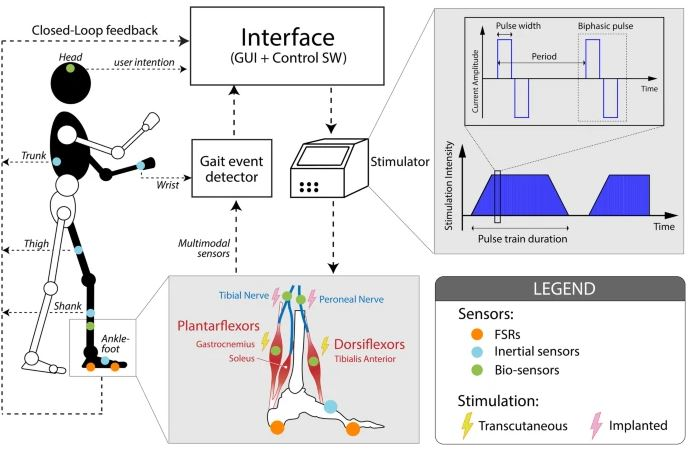
\includegraphics[scale=0.8]{esquema_FES}
  \caption{Arquitectura de una neuroprótesis para pie caído en lazo cerrado. Se utilizan sensores para detectar la fase del ciclo de marcha y estimular eléctricamente en consecencia\cite{estado_arte_FES}.}\label{fig:esquema_FES}
\end{figure}

Prosiguiendo con el análisis de la mencionada revisión, ésta lleva a cabo una clasificación de neuroprótesis para pie caído según diferentes parámetros. Antes de entrar en detalle en dicha clasificación, se ha de mencionar que esta revisión recoge publicaciones que tratan avances tecnológicos en cuanto a diseño y arquitectura de control, así como resultados clínicos provenientes de este tipo de prótesis. Para ello, se tienen en cuenta publicaciones en las bases de datos de PubMed, PEDro, SCOPUS, Academic Google, MEDLINE, EMBASE, ResearchGate, WoS, and SciELO. Además, se tienen como criterios de búsqueda publicaciones entre los años 2000 y 2018, estudios que presenten neuroprótesis para pie caído, estudios presentados en revistas o conferencias, tesis o catálogos y se excluyen todos los estudios que traten sobre prótesis híbridas.
\\
\\
Siguiendo con la clasificación mencionada previamente, esta revisión del estado del arte crea dos grupos de neuroprótesis según su tipo de control: lazo abierto y lazo cerrado. Además, independientemente del tipo de control se crea otra clasificación según el tipo de sensores embarcados en la neuroprótesis: resistivos, inerciales y biosensores. Además, como categorías secundarias, se diferencia entre neuroprótesis para investigación o comercial, transcutánea o implantada y se especifica su número de canales así como el tipo de movimiento en el que asiste al paciente. De este modo, se recoge en la figura \ref{fig:clasificacion_estado_arte_FES} todas las neuroprótesis encontradas acorde los criterios de búsqueda y clasificadas según los parámetros mencionados.\\

\begin{figure}[!htb]
\centering
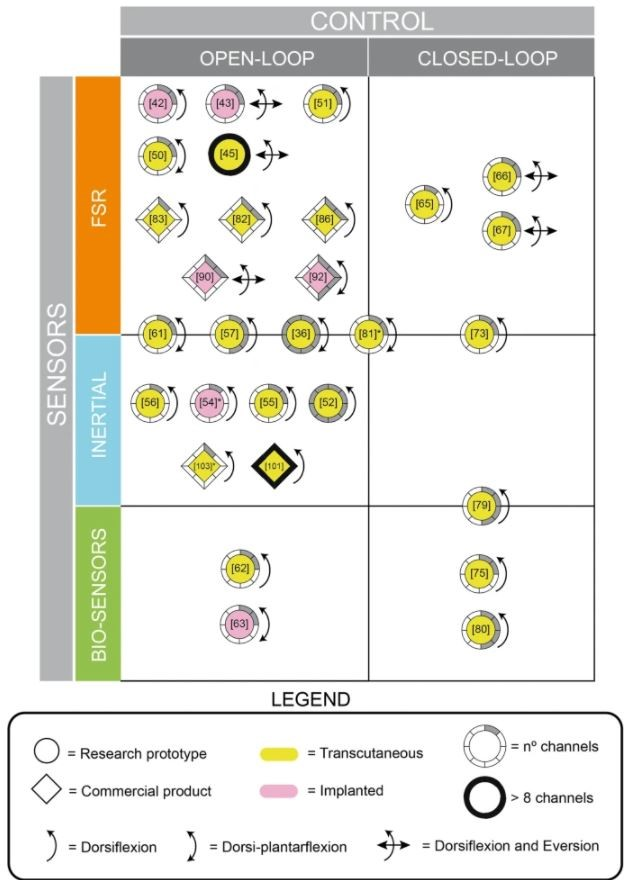
\includegraphics[scale=0.8]{clasificacion_estado_arte_FES}
  \caption{Clasificación de neuroprótesis para pie caído\cite{estado_arte_FES}.}\label{fig:clasificacion_estado_arte_FES}
\end{figure}

La revisión estudia todas las neuroprótesis expuestas en la figura anterior las cuales no se van a exponer en el presente trabajo por cuestiones de brevedad. Sin embargo, es importante destacar las conclusiones de dicha revisión ya que supone una puesta en común de fortalezas y debilidades de este tipo de prótesis además de plantear directrices y vías de mejora. 
\\
\\
En primer lugar, es importante destacar que se han hecho progresos importantes durante las últimas dos décadas en cuanto a la arquitectura de las neuroprótesis y las estrategias para obtener mejores resultados en la neuro-rehabilitación. De hecho, muchas de ellas tienen uso comercial, es decir, fuera de laboratorios y centros especializados para dotar de mayor libertad al paciente que las necesite. Sin embargo, todavía existen limitaciones en el uso de este tipo de prótesis siendo la principal de ellas la fatiga muscular provocada por la electroestimulación de forma continuada y la cual debe gestionarse. Además, se ha observado una falta en el desarrollo de sistemas bilaterales, es decir, para asistir ambas extremidades. 
\\
\\
Como vías de mejora, es importante desarrollar la estrategia de assist-as-need (AAN), mencionada con anterioridad en este capítulo, además del control en lazo cerrado el cual permite una neuro-reahabilitación dinámica e individualizada. Otra rama de desarrollo implica el uso de electrodos transcutáneos con un ajuste automático, lo cual permite utilizar la neuroprótesis fuera de clínicas y centros especializados. Esto permite una mayor adaptación segura del ciclo de marcha en diferentes entornos de la vida diaria como pueden ser escaleras o superficies inclinadas. En cuanto a las técnicas de electroestimulación, la combinación de pulsos de frecuencia constante (CFT) y frecuencia variable (VFT) es prometedora en cuanto a la reducción de fatiga muscular. Por último, se considera de gran importancia el desarrollo de estudios de largo alcance para la medición de la actividad muscular durante la marcha para una mejor comprensión y cuantificación de los mecanismos implicados en el ciclo de marcha y neuro-rehabilitación de cada paciente.


\section{Objetivos del trabajo}
Tal y como se ha mencionado en el presente capítulo, el autor del trabajo lo ha realizado en el grupo de neuro-rehabilitación del Instituto Cajal. Dicho grupo desarrolla un proyecto que tiene lugar en un ámbito de investigación de la neuro-rehabilitación de la marcha patológica en continuo desarrollo. Se parte de la idea del uso de sistemas neuro-mecánicos (electroestimulación en conjunto a sistemas mecánicos como un exoesqueleto) para unificar sus ventajas y minimizar sus limitaciones. Esta combinación resulta más ventajosa que utilizar cualquiera de sus componentes por separado, tal y como se vio en el apartado \ref{protesis_hibridas}. De hecho, se puede incluso conseguir que pacientes con paraplejia sean capaces de levantarse o sentarse, caminar y subir o bajar escaleras.
\\
\\
Teniendo en cuenta el marco en el que se sitúa el presente Trabajo Fin de Máster, se procede a explicar cómo encaja en el equipo de neuro-rehabilitación y su objetivo final. El proyecto que desarrolla el equipo se centra en la neuro-rehabilitación de la marcha patológica debida a daños en el sistema nervioso central causados por lesiones medulares e ictus\cite{tesis_antonio}. Para ello, está desarrollando una prótesis híbrida cuyos componentes son los siguientes:

\begin{itemize}
\item[•] Un exoesqueleto robótico capaz de generar movimiento
\item[•] Neuroprótesis modular para el control neuromuscular en red mediante electroestimulación funcional o FES
\item[•] Conjunto de sensores 
\end{itemize}

Además, se está desarrollando un subproyecto del anterior con los siguientes objetivos:
\begin{itemize}
\item[•] Diseño y desarrollo de la neuroprótesis modular
\item[•] Integración de la neuroprótesis con el exoesqueleto 
\item[•] Validación de la neuroprótesis para su aplicación en control híbrido con el exoesqueleto
\end{itemize}

La neuroprótesis, tal y como se ha mencionado, es modular lo que significa que se puede hacer uso de hasta cuatro dispositivos de electroestimulación independientes. Estos se explicarán en mayor detalle en el siguiente capítulo así como el resto de componentes de la neuroprótesis. Sin embargo, cabe destacar en este punto que se pretende efectuar un control y configuración de la prótesis híbrida desde un ordenador de forma inalámbrica, para mayor comodidad y flexibilidad en la neuro-rehabilitación de la marcha patológica. 
\\
\\
\textbf{El autor del presente Trabajo Fin de Máster participa tanto en el proyecto principal como en el subproyecto y colabora en todos los objetivos expuestos. Por tanto, las contribuciones al proyecto y objetivos del trabajo son:}

\begin{itemize}
\item[\textbf{1)}] \textbf{Selección y programación de un microcontrolador para el control centralizado de la prótesis híbrida con las siguientes funciones:}
\begin{itemize}
\item[a)] Recibir y procesar las mediciones arrojadas por el exoesqueleto y el conjunto de sensores utilizado.

\item[b)] Controlar de forma simultánea y en tiempo real hasta cuatro dispositivos de electroesimulación en función de la información recibida por los sensores. Esto implica modificar el comportamiento de los dispositivos de estimulación durante la realización del ejercicio de rehabilitación.

\item[c)] Controlar en tiempo real el exoesqueleto en función del estado de los electroestimuladores y las mediciones de los sensores.


\end{itemize}
\item[\textbf{2)}] \textbf{Desarrollo de una interfaz gráfica de usuario para para:}
\begin{itemize}
\item[a)] Establecer una configuración inicial de la prótesis para la tarea de rehabilitación correspondiente así como cargar y guardar perfiles de configuración. Esto se lleva a cabo mediante una comunicación directa entre la interfaz y el microcontrolador expuesto en el punto 1).

\item[b)] Visualizar en tiempo real las mediciones del conjunto de sensores utilizado.

\item[c)] Controlar el ejercicio de rehabilitación iniciando o deteniendo la transmisión de datos de los sensores y el exoesqueleto así como la estimulación eléctrica.
\end{itemize}


\item[\textbf{3)}] \textbf{Revisión y mejora del hardware de los módulos de la neuroprótesis:}
\begin{itemize}
\item[a)] Revisión y mejora de las tarjetas de circuito impreso correspondientes a las etapas de control y potencia.
\end{itemize}

\item[\textbf{4)}] \textbf{Revisión y mejora del software de los módulos de la neuroprótesis:}
\begin{itemize}
\item[a)] Optimización de la comunicación con el dispositivo.
\end{itemize}
\end{itemize}

Una vez expuestos los objetivos del presente Trabajo Fin de Máster, se muestra en la figura \ref{fig:esquema_protesis_objetivos} un esquema generalizado de la prótesis híbrida en cuyo desarrollo participa el autor del trabajo y que supone el objetivo global del mismo. Se aprecia cómo el microcontrolador actúa de nodo central entre el exoesqueleto, electroestimuladores y sensores así cómo éste es accesible con un ordenador desde la interfaz gráfica de usuario mencionada previamente. No se pretende en este punto explicar en detalle el esquema ya que deben tratarse características tales como los protocolos de comunicación y propiedades del microcontrolador y resto de componentes de la prótesis. Dichos detalles se verán en su correspondiente capítulo.\\

\begin{figure}[!htb]
\centering
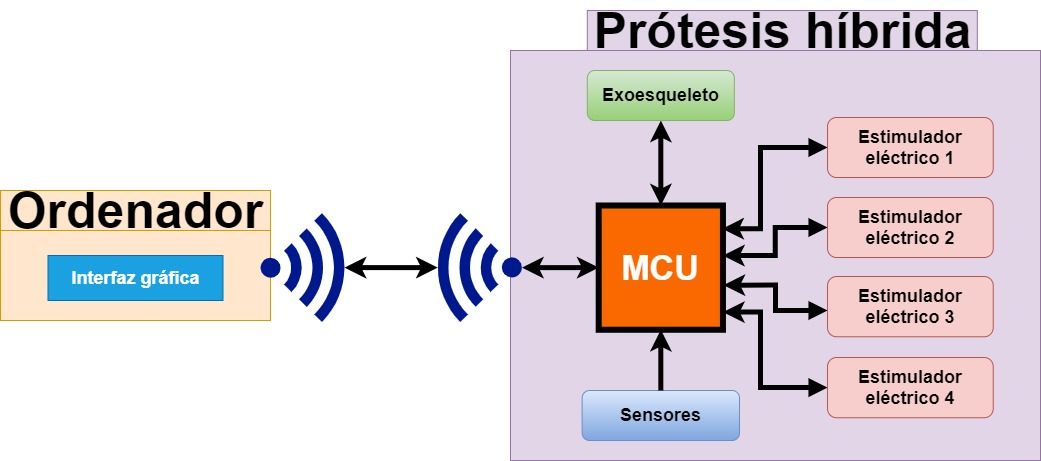
\includegraphics[scale=0.4]{esquema_protesis_objetivos}
  \caption{Esquema simplificado de la prótesis híbrida. Las flechas indican la comunicación entre los elementos unidos, bidireccional o unidireccional, sin especificar el protocolo.}\label{fig:esquema_protesis_objetivos}
\end{figure}

